\documentclass[a4paper,oneside,DIV=9,fontsize=12pt]{scrartcl}

\usepackage{fontspec,unicode-math}
\setromanfont{PT Serif}
\setsansfont{PT Sans}
\setmonofont{PT Mono}
\setmathfont{STIX Two Math}

\usepackage{microtype}

\usepackage{polyglossia}
\setdefaultlanguage{ukrainian}
\PolyglossiaSetup{ukrainian}{indentfirst=true}
\setotherlanguage{english}

\usepackage[inline]{enumitem}

\usepackage{tikz}
\usetikzlibrary{graphs,quotes}

\usepackage{booktabs}

\usepackage{algorithm}
\usepackage{algpseudocode}

\begin{document}
	\section{Дискретна математика}
		\subsection{Визначити поняття істинності складного логічного вислову як функції значень істинності двох простих висловів}
			Булевою функцією називається функція вигляду $f : E^n \rightarrow E$, де $E = {0, 1}$, тобто $f(x_1, x_2, \dots, x_n)$, що приймає значення 0, 1 та аргументи якої можуть приймати значення 0, 1.
		
		\subsection{Визначити поняття множини і два способи подання множин, проілюструвавши це прикладами}
			Множина --- аксіоматичне, початкове поняття, тому апріорі не може мати формального визначення. Основоположник теорії множин Георг Кантор дає таке визначення: «Під поняттям „множина“ ми розуміємо об'єднання у деяке ціле $M$ певних добре відрізняємих предметів $m$ нашого спостереження або мислення, які будуть називатись елементами множини $M$».
		
			Множина --- це сукупність певних відрізняючихся об'єктів таких, що для будь-якого об'єкта можна встановити, чи належить він даній множині.
		
			Множина складається з елементів. Належність елемента $a$ до множини $M$ позначається $a \in M$. Неприналежність позначається $a \notin M$.
		
			Множина може бути задана перерахуванням (списком своїх елементів), породжуючою процедурою або описом характерних властивостей, які мають його елементи.
		
			Списком можна задавати лише скінченні множини. Наприклад, запис $A = {a, b, d, h}$ означає, що множина $A$ складається з елементів $a, b, d, h$.
		
			Породжуюча процедура описує спосіб отримання елементів множини з уже отриманих елементів чи інших об'єктів. Елементами множини вважаються усі об'єкти, що можуть бути отримані за допомогою такої процедури. Наприклад, нехай множина $M_4$ містить усі числа виду $\pi \div 2 \pm k\pi$, де $k \in N_0$. Або, нехай є множина $M_{2^n} = {1, 2, 4, 8, 16 \dots}$, то її породжуюча процедура визначається за такими правилами:
			\begin{enumerate*}
				\item $1 \in M_{2^n}$
				\item Якщо $m \in M_{2^n}$, то $2m \in M_{2^n}$
			\end{enumerate*}.
		
		\subsection{Визначити поняття орієнтованого і неорієнтованого графа і навести приклади їх застосування для опису відношень між об'єктами довільної системи.}
			Сучасна теорія графів не має усталеної термінології, тому у різних підручниках визначення понять можуть відрізнятись.
			
			Граф --- це сукупність двох множин: $V$ (точок) та $E$ (ліній), між елементами яких визначено відношення \emph{інцидентності}, при чому кожен елемент $e \in E$ інцидентний рівно двом елементам $v', v'' \in V$. Елементи множини $V$ називають вершинами графа $G$, елементи множини $E$ --- його ребрами. Вершини та ребра графа $G$ ще називають його елементами, та записують $v \in G$, $e \in G$.
			
			У деяких задачах інцидентні ребру вершини розглядаються у певному порядку, тоді кожному ребру можна приписати напрям з одної інцидентної вершини в іншу. Направлені ребра можуть називати \emph{дугами}.
			
			Граф --- це упорядкована пара $G = (V, E$) множин, що задовольняють $E \subseteq \left[V\right]^2$, тобто елементи множини $E$ є двоелементними підмножинами $V$. Якщо $E$ --- множина неупорядкованих пар, то граф $G$ є неорієнтованим, якщо ж $E$ --- множина упорядкованих пар, то граф $G$ --- орієнтований.
			
			За допомогою графів можна зобразити соціальну мережу, де вершинами є люди, а ребрами --- зв'язки між ними. Графи часто використовуються у комп'ютерних науках: для зображення скінченних автоматів, структур даних, блок-схем, ієрархії файлової системи, графів програм тощо.
			
		\subsection{Визначити способи представлення неорієнтовних графів за допомогою двох графоутворюючих множин --- множини вершин $X$ і множини ребер $Y$ --- за допомогою матриці суміжності.}
			Матриця суміжності графа --- це квадратна матриця $\left|\left|\delta_{ij}\right|\right|$, де рядками та стовпчиками є вершини графа. Для неорієнтованого графа $\delta_{ij}$ дорівнює кількості ребер, інцидентних $i$-тій та $j$-тій вершинам. Таким чином, матриця суміжності неорієнтованого графа симетрична. Орієнтований граф з симетричною матрицею суміжності канонічно відповідає неорієнтованому графу, що має таку ж матрицю суміжності.
			
			Нехай є граф $G = (X, Y)$, зображений на рис. \ref{fig:unidirgraph}, $X = \{v_1, v_2, v_3, v_4\}$, $Y = \{e_1, e_2, e_3, e_4\}$, тоді його матриця суміжності наведена у табл. \ref{tab:gadjmatrix}.
			
			\begin{figure}[h!]
				\centering
				
				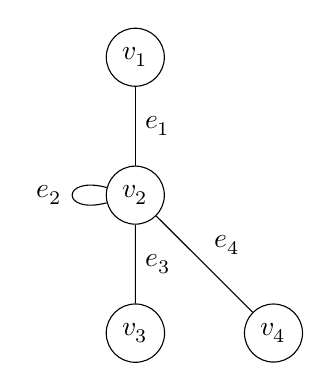
\begin{tikzpicture}[every loop/.style={}]
					\graph [math nodes, nodes={draw, circle}, grow down sep=1cm, branch right sep=1cm]
					{ "v_1" --["$e_1$"] "v_2" --[loop left, "$e_2$"] "v_2" -- {"v_3" [> "$e_3$"], "v_4" [> "$e_4$"]} };
				\end{tikzpicture}
				
				\caption{Граф $G$}
				\label{fig:unidirgraph}
			\end{figure}
			
			\begin{table}[h!]
				\centering
				
				\begin{tabular}{lllll}
					\toprule
						      & $v_1$ & $v_2$ & $v_3$ & $v_4$ \\
						$v_1$ & 0     & 1     & 0     & 0     \\
						$v_2$ & 1     & 1     & 1     & 1     \\
						$v_3$ & 0     & 1     & 0     & 0     \\
						$v_4$ & 0     & 1     & 0     & 0     \\
					\bottomrule
				\end{tabular}
				
				\caption{Матриця суміжності графа $G$}
				\label{tab:gadjmatrix}
			\end{table}
			
		\subsection{Визначити способи представлення неорієнтовних графів за допомогою двох графоутворюючих множин --- множини вершин $X$ і множини ребер $Y$ --- за допомогою матриці інциденцій.}
			Нехай є скінченний граф $G = (X, Y)$, $X = \{v_1, \dots v_n\}$, $Y = \{e_1, \dots e_m\}$. Матриця інциденцій --- це матриця $||\varepsilon_{ij}||$, яка має $m$ рядків і $n$ стовпчиків. Відповідність між стовпчиками, рядками, вершинами та ребрами залежить від переваги автора. Зазвичай стовпчики відповідають ребрам, а рядки --- вершинам (за Кузнєцовим стовпчики відповідають вершинам графа, рядки --- ребрам). Якщо ребро $e_i$ інцидентно вершині $v_i$, то $\varepsilon_{ij} = 1$, інакше $\varepsilon_{ij} = 0$.
			
			Для графа на рис. \ref{fig:unidirgraph} матриця інциденцій зображена на табл. \ref{tab:unidirinctable}.
			
			\begin{table}[h!]
				\centering
				
				\begin{tabular}{lllll}
					\toprule
					      & $e_1$ & $e_2$ & $e_3$ & $e_4$\\
					$v_1$ & 1     & 0     & 0     & 0    \\
					$v_2$ & 1     & 1     & 1     & 1    \\
					$v_3$ & 0     & 0     & 1     & 0    \\
					$v_4$ & 0     & 0     & 0     & 1    \\
					\bottomrule
				\end{tabular}
				
				\caption{Матриця інциденцій графа на рис. \ref{fig:unidirgraph}}
				\label{tab:unidirinctable}
			\end{table}
			
		\subsection{Визначити способи представлення орієнтовних графів за допомогою двох графоутворюючих множин --- множини вершин $X$ і множини дуг $Y$ --- за допомогою матриці суміжності.}
			Матриця суміжності графа --- це квадратна матриця $\left|\left|\delta_{ij}\right|\right|$, де рядками та стовпчиками є вершини графа. Для орієнтованого графа цей елемент матриці суміжності дорівнює кількості ребер з початком в $i$-тій вершині та кінцем в $j$-тій. Таким чином, матриця суміжності орієнтованого графа необов'язково симетрична. Якщо матриця суміжності орієнтованого графа симетрична, це означає, що для кожного ребра існує ребро, що з'єднує ті ж самі вершини у протилежному напрямку. Орієнтований граф з симетричною матрицею суміжності канонічно відповідає неорієнтованому графу, що має таку ж матрицю суміжності.
			
			Нехай є граф $G = (X, Y)$, зображений на рис. \ref{fig:dirgraph}, $X = \{v_1, v_2, v_3, v_4\}$, $Y = \{e_1, e_2, e_3, e_4\}$, тоді його матриця суміжності наведена у табл. \ref{tab:dirgadjmatrix}.
			
			\begin{figure}[h!]
				\centering
				
				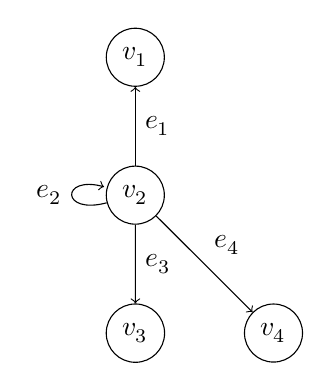
\begin{tikzpicture}
					\graph [math nodes, nodes={draw, circle}, grow down sep=1cm, branch right sep=1cm]
					{ "v_1" <-["$e_1$"] "v_2" ->[loop left, "$e_2$"] "v_2" -> {"v_3" [> "$e_3$"], "v_4" [> "$e_4$"]} };
				\end{tikzpicture}
				
				\caption{Граф $G$}
				\label{fig:dirgraph}
			\end{figure}
			
			\begin{table}[h!]
				\centering
				
				\begin{tabular}{lllll}
					\toprule
						      & $v_1$ & $v_2$ & $v_3$ & $v_4$ \\
						$v_1$ & 0     & 0     & 0     & 0     \\
						$v_2$ & 1     & 1     & 1     & 1     \\
						$v_3$ & 0     & 0     & 0     & 0     \\
						$v_4$ & 0     & 0     & 0     & 0     \\
					\bottomrule
				\end{tabular}
				
				\caption{Матриця суміжності графа $G$}
				\label{tab:dirgadjmatrix}
			\end{table}
		
		\subsection{Визначити способи представлення орієнтовних графів за допомогою двох графоутворюючих множин --- множини вершин $X$ і множини ребер $Y$ --- за допомогою матриці інциденцій.}
			Нехай є скінченний орієнтований граф $G = (X, Y)$, $X = \{v_1, \dots v_n\}$, $Y = \{a_1, \dots a_m\}$. Матриця інциденцій --- це матриця $||\varepsilon_{ij}||$, яка має $m$ рядків і $n$ стовпчиків. Відповідність між стовпчиками, рядками, вершинами та ребрами залежить від переваги автора. Зазвичай стовпчики відповідають ребрам, а рядки --- вершинам (за Кузнєцовим стовпчики відповідають вершинам графа, рядки --- ребрам). Якщо вершина $v_i$ --- початок ребра $a_i$, то $\varepsilon_{ij} = -1$; якщо $v_i$ --- кінець ребра $a_i$, то $\varepsilon = 1$; якщо $a_i$ --- петля, а $a_i$ --- інцидентна їй вершина, то $\varepsilon_{ij} = \alpha$, де $\alpha$ --- будь-яке число, відмінне від −1, 0, 1; в усіх інших випадках $\varepsilon_{ij} = 0$.
			Для графа на рис. \ref{fig:dirgraph} матриця інциденцій наведена у табл. .
			
			\begin{table}[h!]
				\centering
				
				\begin{tabular}{lllll}
					\toprule
						      & $e_1$ & $e_2$ & $e_3$ & $e_4$ \\
						$v_1$ & 1     & 0     & 0     & 0     \\
						$v_2$ & −1    & 2     & −1    & −1    \\
						$v_3$ & 0     & 0     & 1     & 0     \\
						$v_4$ & 0     & 0     & 0     & 1     \\
					\bottomrule
				\end{tabular}
				
				\caption{Матриця інциденцій графа}
			\end{table}
		
		\subsection{Навести правила де Моргана об’єднання і перерізу двох множин.}
			$\overline{A \cup B} = \overline{A} \cap \overline{B}$, $\overline{A \cap B} = \overline{A} \cup \overline{B},$ де $A$, $B$ --- множини, $\overline{A}$ --- доповнення множини $A$.
		
		\subsection{Скласти таблицю істинності для двох простих логічних висловів $A$ і $B$, над якими проводиться операції заперечення, диз'юнкції, кон'юнкції, імплікації та подвійної імплікації.}
			\begin{table}[h!]
				\centering
				
				\begin{tabular}{cccccccc}
					\toprule
					$A$ & $B$ & $\lnot A$ & $\lnot B$ & $A \land B$ & $A \lor B$ & $A \rightarrow B$ & $A \leftrightarrow B$ \\
					\midrule
					 0  & 0   & 1         & 1         & 0           & 0          & 0                 & 1\\
					 0  & 1   & 1         & 0         & 0           & 1          & 0                 & 0\\
					 1  & 0   & 0         & 1         & 0           & 1          & 1                 & 0\\
					 1  & 1   & 0         & 0         & 1           & 1          & 0                 & 1 \\	
					\bottomrule
				\end{tabular}
			\end{table}
		
	\section{Алгоритми та методи обчислень}
		\subsection{Області застосування алгоритмів}
		
		\subsection{Властивості алгоритмів}
			За <<Мистецтвом програмування>> Д.~Кнута, алгоритми мають п'ять важливих властивостей:
			\begin{enumerate}
				\item Скінченність --- алгоритм завжди повинен завершувати роботу після скінченної кількості кроків. Процедура, що має усі властивості алгоритму, крім скінченності, може називатись \emph{обчислювальним методом}.
				\item Визначеність --- кожен крок алгоритму повинен бути точно визначений; дії, що мають бути виконані, повинні бути точно і однозначно визначені.
				\item Вхідні дані --- алгоритм має нуль або більше вхідних даних. Дані надаються алгоритму до початку його роботи або під час виконання. Ці вхідні дані беруться з певного набору об'єктів.
				\item Вихідні дані --- алгоритм має одне або більше вихідних даних: значень, що мають задане відношення до вхідних даних.
				\item Ефективність --- усі операції, що описані в алгоритмі, повинні бути достатньо простими для того, щоб бути точно виконаними та за скінченну кількість часу на папері.
			\end{enumerate}
			
		\subsection{Відсортувати заданий масив методом вставки та <<бульбашки>>}
			Метод вставки:
			
			\begin{algorithm}
				\caption{Алгоритм сортування вставкою}
				
				\begin{algorithmic}[1]
					\For{j = 2 to A.length}
						\State $key = A[j]$
						\State $i = j - 1$
						\While{$i > 0$ and $A[i] > key$}
							\State $A[i+1] = A[i]$
							\State $i = i - 1$
						\EndWhile
						\State $A[i+1] = key$
					\EndFor
				\end{algorithmic}
				
			\end{algorithm}
			
			Метод бульбашки.
	\section{Програмування}
\end{document}